%!TEX program = xelatex
% 完整编译: xelatex -> bibtex -> xelatex -> xelatex
\documentclass[lang=cn,11pt,a4paper]{elegantpaper}
%\usepackage{showframe}
\usepackage{multirow}
\title{工程伦理的未来研究方向:微观伦理学,宏观伦理学和专业协会的角色}
\author{Joseph R. Herkert}
\institute{North Carolina State University, USA}

\version{}
\date{}


\begin{document}

\maketitle

\begin{abstract}
本文讨论三个工程伦理中框架——个人、专业和协会——这可以进一步分为关注个人和工程行业的内部关系的“微观伦理”和关注工程领域的集体社会责任和社会技术决策的“宏观伦理”。很少有人尝试将微观伦理和宏观伦理方法整合到工程伦理中。本文建议的方法是着重于专业工程协会在联系个人和专业伦理以及在联系专业和社会伦理方面的作用。前者的例子是用伦理支持概述了一个研究项目,后者以产品责任立场声明的发布为例。
\keywords{伦理支持,宏观伦理,产品责任,专业协会,公共政策,工程伦理的研究} 
\end{abstract}



\section{工程中的微观伦理和宏观伦理}
许多作者认为工程伦理包含多个领域。伦理学家John Ladd将工程伦理学细分为“微观伦理学”或“宏观伦理学”,这取决于关注的焦点是工程师个人与客户、同事和雇主之间的关系,或者该职业的集体社会责任。在每一个案例中,Ladd似乎都关心所谓的“职业道德”,微观道德主要关注职业内部的问题,而宏观道德则关注更广泛的社会背景下的职业责。

作为一名工程师,McLean在讨论工程伦理学时运用了三个范畴:处理工程师技术决策的技术伦理;处理经理、工程师和雇主之间的关系的职业伦理和处理与技术相关的社会政治决策的社会伦理。McLean的职业道德概念比Ladd更狭隘,只包含了Ladd所描述的微观道德的那些维度。与此同时,McLean对与工程相关的道德领域有一个比Ladd更广泛的总体概念,因为他包括个人和社会两个方面。

另一位工程师Vanderburg虽然使用了与Ladd类似的术语,
在区分“个体技术或从业者”的“微观层面”分析和“整体技术”的“宏观层面”分析时,似乎完全忽视了职业道德类别。范德堡的分类与另一位工程师Devon相似,他提出了一种新的工程伦理范式,他称之为“社会伦理”,包括与技术相关的“专业知识的社会关系”管理和决策,而不是关注个人。

De George是一位伦理学家,他对“工程伦理学”和“伦理学”进行了区分工程。前者关注的是个人的行为,而后者关注的是专业内部的关系和工程专业对社会的责任。De George的“工程伦理”概念因此融合了Ladd的微观和宏观维度。此外,“工程伦理”还具体包括专业工程学会。

如表1所示,在梳理工程伦理的这些不同方面时,出现了一个有趣的模式。三个显而易见的参考框架是:个人、专业和社会。结合Ladd和Vanderburg的术语,“微观伦理学”可以被视为包括对个人和工程专业内部关系的关注,而“宏观伦理学”既适用于工程专业的集体社会责任,也适用于关于技术的社会决策。
\section{研究的问题}
迄今为止,大多数工程伦理学的研究和教学都有一个微观的焦点,要么是Vanderburg使用的术语,要么是Ladd使用的术语。政治哲学家兰登·温纳(Langdon Winner)对这种情况表示遗憾,他批评工程伦理学过分强调微观伦理困境的案例研究,而忽视了与技术发展相关的更大的问题:
\begin{quotation}
  伦理责任……不仅仅是过一种体面的、诚实的、真实的生活,这样的生活当然还是很重要的。当这些选择突然、意外地出现时,它所涉及的远不止是做出明智的选择。我们的道德义务必须……包括愿意让他人参与艰难的工作,以确定技术社会面临的关键选择是什么,以及如何明智地应对这些选择。
\end{quotation}

% Please add the following required packages to your document preamble:
% \usepackage{multirow}
% Please add the following required packages to your document preamble:
% \usepackage{multirow}

\begin{table}[htbp]

  \centering
  \caption{工程中的微观伦理和宏观伦理}
  %\resizebox{\textwidth}{!}{
 
  \begin{tabular}{|l|p{2.5cm}|p{3cm}|p{3cm}|p{2.5cm}|}
    \hline
    \multirow{2}{*}{来源} & \multicolumn{2}{l|}{微观伦理} & \multicolumn{2}{l|}{宏观伦理} \\ \cline{2-5} 
                        & 个体          & \multicolumn{2}{l|}{}     & 社会          \\ \hline
    Ladd(1980)          &             & 微观伦理——专业人员与客户、同事和雇主之间的专业关系         & 宏观伦理——一个职业的成员作为一个群体所面临的与社会的关系问题(即专业人士的社会责任)          &             \\ \hline
    McLean(1993)        & 技术伦理——工程师做出的技术决定和判断          & 专业伦理——工程师与其他群体(如经理、工程师、雇主)之间的职业道德互动          &             & 社会伦理——社会层面的技术政策决策          \\ \hline
    Vanderburg(1995)    & 微观分析——个体技术或从业者的微观层次分析          &             &             & 宏观分析——整体技术的宏观层面分析          \\ \hline
    Devon(1999)         & 个体伦理          &             &             & 社会伦理——社会伦理与技术管理和决策有关的“专业知识的社会关系”          \\ \hline
    De George(1993)     & 工程中的伦理——工程师个人工程行为的道德规范          & \multicolumn{2}{p{6cm}|}{工程中的伦理——工程道德工程师在工业和其他组织、专业工程协会中的作用,以及该职业的责任}   &             \\ \hline
  \end{tabular}
  %}
\end{table}


最近,学者们开始讨论与工程有关的宏观伦理问题。然而,还有待开发的是整合微观伦理和宏观伦理方法的综合框架。开发这样一个框架的一个方法是把重点放在专业协会的角色在弥合microethical和macroethical问题建议在德乔治的“道德工程”的概念(见表1)。除了颁布伦理准则,工程专业的专业工程协会的作用已经在很大程度上被忽视了。一些作者,包括Layton12和Unger,13已经认真对待专业协会的作用,但他们的工作大部分集中在专业协会如何连接职业道德的内部和社会责任维度(尽管如下所述,Unger也讨论了道德支持)

此模板基于 \LaTeX{} 的标准文类 article 设计,所以 article 文类的选项也能传递给本模板,比如 \lstinline{a4paper, 11pt} 等等。本模板支持 \hologo{pdfLaTeX} 和 \hologo{XeLaTeX} 编译。

\begin{lstlisting}
\documentclass[a4paper,11pt]{elegantpaper}
\end{lstlisting}

\textbf{注意}:Elegant\LaTeX{} 系列模板已经全部上传至 \href{https://www.overleaf.com/latex/templates/elegantpaper-template/yzghrqjhmmmr}{Overleaf} 上,用户可以在线使用。另外,为了方便国内用户,模板也已经传至\href{https://gitee.com/ElegantLaTeX/ElegantPaper}{码云}。


\subsection{全局选项}
此模板定义了一个语言选项 \lstinline{lang},可以选择英文模式 \lstinline{lang=en}(默认)或者中文模式 \lstinline{lang=cn}。当选择中文模式时,图表的标题引导词以及参考文献,定理引导词等信息会变成中文。你可以通过下面两种方式来选择语言模式:
\begin{lstlisting}
\documentclass[lang=cn]{elegantpaper} % or
\documentclass{cn}{elegantpaper} 
\end{lstlisting}

\textbf{注意:} 英文模式下,由于没有添加中文宏包,无法输入中文。如果需要输入中文,可以通过在导言区引入中文宏包 \lstinline{ctex} 或者加入 \lstinline{xeCJK} 宏包后自行设置字体。 
\begin{lstlisting}
\usepackage[UTF8,scheme=plain]{ctex}
\end{lstlisting}

\subsection{英文与数学字体}

本模板使用 \lstinline{newtxtext} 和 \lstinline{newtxmath} 分别设置全文的英文文本字体和数学字体。数学字体的效果如下:
\begin{equation}
(a+3b)^{n} = \sum_{k=0}^{n} C_{n}^{k} a^{n-k} (3b)^k\label{eq:binom}
\end{equation}

\subsection{自定义命令}
此模板并没有修改任何默认的 \LaTeX{} 命令或者环境\footnote{目的是保证代码的可复用性,请用户关注内容,不要太在意格式,这才是本工作论文模板的意义。}。另外,我自定义了 4 个命令:
\begin{enumerate}
  \item \lstinline{\email}:创建邮箱地址的链接,比如 \email{ddswhu@outlook.com};
  \item \lstinline{\figref}:用法和 \lstinline{\ref} 类似,但是会在插图的标题前添加 <\textbf{图 n}> ;
  \item \lstinline{\tabref}:用法和 \lstinline{\ref} 类似,但是会在表格的标题前添加 <\textbf{表 n}>;
  \item \lstinline{\keywords}:为摘要环境添加关键词。
\end{enumerate}

\subsection{参考文献}
此模板使用 \hologo{BibTeX} 来生成参考文献,中文模式下默认使用的文献样式(bib style)是 \lstinline{GB/T 7714-2015}\footnote{通过调用 \href{https://ctan.org/pkg/gbt7714}{\lstinline{gbt7714}} 宏包}。参考文献示例:~\cite{en3} 使用了中国一个大型的 P2P 平台(人人贷)的数据来检验男性投资者和女性投资者在投资表现上是否有显著差异。

你可以在谷歌学术,Mendeley,Endnote 中获得文献条目(bib item),然后把它们添加到 \lstinline{wpref.bib} 中。在文中引用的时候,引用它们的键值(bib key)即可。注意需要在编译的过程中添加 \hologo{BibTeX} 编译。

本模板还添加了 \lstinline{cite=numbers} 、\lstinline{cite=super} 和 \lstinline{cite=authoryear}  三个参考文献选项,用于设置参考文献格式的设置,默认为 \lstinline{numbers}。理工科类一般使用数字形式 \lstinline{numbers} 或者上标形式 \lstinline{super},而文科类多使用作者-年份 \lstinline{authoryear} 比较多。如果需要改为 \lstinline{cite=numbers}  或者  \lstinline{authoryear} ,可以使用
\begin{lstlisting}
\documentclass[cite=super]{elegantpaper} % super style ref style
\documentclass[super]{elegantpaper}

\documentclass[cite=authoryear]{elegantpaper} % author-year ref style
\documentclass[authoryear]{elegantpaper}
\end{lstlisting}


\section{协作人员招募}
招募 Elegant\LaTeX{} 的协作人员,没有工资。工作内容:翻译 Elegant\LaTeX{} 系列模板相关的文稿(中翻英),维护模板的 wiki(主要涉及 Markdown),如果有公众号文稿写作经历的话,也可以帮忙写微信稿。本公告长期有效。

目前 ElegantLaTeX 共有 4 名协作人员,分别是
\begin{itemize}
  \item 官方文档翻译: \href{https://github.com/peggy2006xzyz}{YPY};
  \item Github 维基维护: \href{https://github.com/izinngo}{Ingo Zinngo}、\href{https://github.com/xiaohao890809}{追寻原风景};
  \item QQ 群管理员: \href{https://github.com/sikouhjw}{Sikouhjw}.
\end{itemize}

在此感谢他们无私的奉献!


\section{致谢}
截止到 2019 年 10 月 17 日,ElegantPaper v0.08 版本发布,ElegantPaper 模板在 Github 上的收藏数(star)达到了 164。在此特别感谢 China\TeX{} 以及 \href{http://www.latexstudio.net/}{\LaTeX{} 工作室}对于本系列模板的大力宣传与推广。

如果你喜欢我们的模板,你可以在 Github 上收藏(Star)我们的模板。
\begin{figure}[htbp]
  \centering
  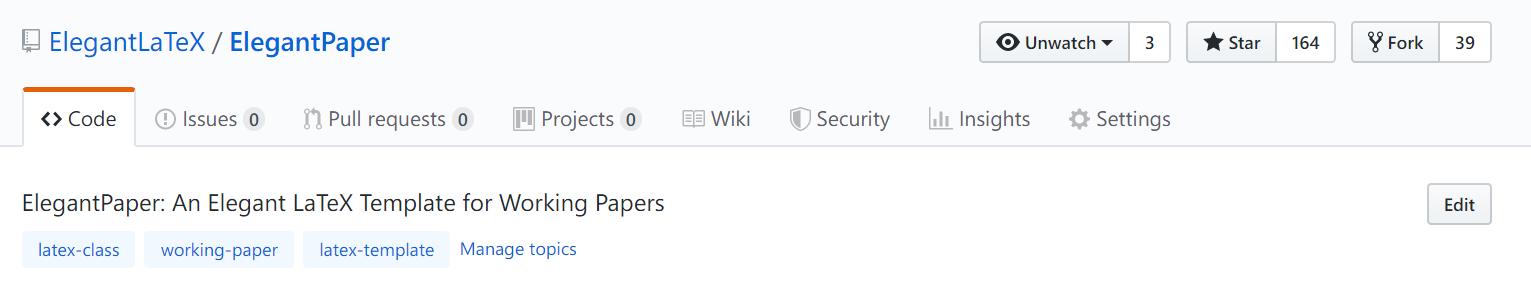
\includegraphics[width=\textwidth]{star.png}
  \caption{一键三连求赞}
\end{figure}

\section{捐赠}
如果您非常喜爱我们的模板,你还可以选择捐赠以表达您对我们模板和我的支持!

\begin{figure}[htbp]
  \centering
  
\includegraphics[width=0.5\textwidth]{donate.jpg}
\end{figure}

\textbf{赞赏费用的使用解释权归 Elegant\LaTeX{} 所有,并且不接受监督,请自愿理性打赏}。10 元以上的赞赏,我们将列入捐赠榜,谢谢各位金主!

\begin{table}[!htbp]
  \centering
  \caption{Elegant\LaTeX{} 系列模板捐赠榜}
  \begin{tabular}{crcc}
    \toprule
    捐赠者   & 金额 & 时间 & 渠道 \\
    \midrule
    Lerh  & 10 元  & 2019/05/15 & 微信 \\
    越过地平线 & 10 元    & 2019/05/15 & 微信 \\
    大熊 &  20 元 & 2019/05/27 & 微信 \\
    * 空 & 10 元 & 2019/05/30 & 微信\\
    \href{http://www.latexstudio.net/}{latexstudio.net} & 666 元 & 2019/06/05 & 支付宝\\
    Cassis & 11 元 & 2019/06/30 & 微信\\
    * 君 & 10 元 & 2019/07/23 & 微信\\
    * 萌 & 19 元 & 2019/08/28 & 微信 \\
    曲豆豆 & 10 元 & 2019/08/28 & 微信 \\
    李博 & 100 元 & 2019/10/06 & 微信\\
    Njustsll & 10 元 & 2019/10/11 & 微信 \\
  \bottomrule
  \end{tabular}%
\end{table}%

\section{常见问题 FAQ}

\begin{enumerate}[label=\arabic*).]
  \item \textit{如何删除版本信息?}\\
      导言区不写 \lstinline|\version{x.xx}| 即可。
  \item \textit{如何删除日期?}\\
      需要注意的是,与版本 \lstinline{\version} 不同的是,导言区不写或注释 \lstinline{\date} 的话,仍然会打印出当日日期,原因是 \lstinline{\date} 有默认参数。如果不需要日期的话,日期可以留空即可,也即 \lstinline|\date{}|。
  \item \textit{如何获得中文日期?}\\
      为了获得中文日期,必须在中文模式下\footnote{英文模式下,由于未加载中文宏包,无法输入中文。},使用 \lstinline|\date{\zhdate{2019/10/11}}|,如果需要当天的汉化日期,可以使用 \lstinline|\date{\zhtoday}|,这两个命令都来源于 \href{https://ctan.org/pkg/zhnumber}{\lstinline{zhnumber}} 宏包。
  \item \textit{如何添加多个作者?}\\
      在 \lstinline{\author} 里面使用 \lstinline{\and},作者单位可以用 \lstinline{\\} 换行。\begin{lstlisting}
\author{author 1\\ org. 1 \and author 2 \\ org. 2 }
\end{lstlisting}
  \item \textit{如何添加中英文摘要?}\\
      请参考 \href{https://github.com/ElegantLaTeX/ElegantPaper/issues/5}{Github::ElegantPaper/issues/5}
\end{enumerate}

\section{示例}

为了让大家更加清楚最终的论文效果,如下给出两篇使用 ElegantPaper 模板排版的工作论文示例,也欢迎大家“投稿”!

\begin{enumerate}
  \item \href{https://github.com/EthanDeng/bank-custody}{银行存管、投资者决策与 P2P 网络借贷规范发展};
  \item \href{https://github.com/EthanDeng/risk-awareness}{互联网金融风险与投资者风险意识 —— 来自网贷平台交易数据的证据}。
\end{enumerate}

这是一个最小示例文档(Minimal Example):
\begin{lstlisting}
\documentclass[lang=cn,a4paper,11pt]{elegantpaper}

% title information
\title{Working Paper Example}
\author{Author Name} 
\institute{Elegant\LaTeX{} Group}

\version{1.00}
\date{\today}

\begin{document}

\maketitle

\begin{abstract}
Your abstract goes here.
\keywords{keyword1, keyword2}
\end{abstract}

\section{Introduction}
The content of introduction section.

\section{Conclusion}
The content of conclusion section.

\bibliography{wpref}

\end{document}
\end{lstlisting}

\nocite{*}
\bibliography{wpref}

\end{document}
